\documentclass{beamer} %[12pt,handout]

\usepackage[english]{babel}
\selectlanguage{english}
\usepackage[utf8]{inputenc}
\usepackage{hyperref}
\usepackage{url}
\usepackage{csvsimple}
\usepackage{bera}% optional: just to have a nice mono-spaced font
\usepackage{listings}
\usepackage{xcolor}
\usepackage{graphicx}
\usepackage{listings}

\colorlet{punct}{red!60!black}
\definecolor{background}{HTML}{EEEEEE}
\definecolor{delim}{RGB}{20,105,176}
\colorlet{numb}{magenta!60!black}

\lstset{basicstyle=\ttfamily,
  showstringspaces=false,
  commentstyle=\color{red},
  keywordstyle=\color{blue},
  breaklines=true,
  postbreak=\raisebox{0ex}[0ex][0ex]{\ensuremath{\color{black}\hookrightarrow\space}},
  morekeywords={run, p, e, v, name,d},
  xleftmargin=-30pt,
  xrightmargin=0pt,
}

\lstdefinelanguage{json}{
    basicstyle=\normalfont\ttfamily,
    numbers=left,
    numberstyle=\scriptsize,
    stepnumber=1,
    numbersep=8pt,
    showstringspaces=false,
    breaklines=true,
    frame=lines,
    backgroundcolor=\color{background},
    literate=
     *{0}{{{\color{numb}0}}}{1}
      {1}{{{\color{numb}1}}}{1}
      {2}{{{\color{numb}2}}}{1}
      {3}{{{\color{numb}3}}}{1}
      {4}{{{\color{numb}4}}}{1}
      {5}{{{\color{numb}5}}}{1}
      {6}{{{\color{numb}6}}}{1}
      {7}{{{\color{numb}7}}}{1}
      {8}{{{\color{numb}8}}}{1}
      {9}{{{\color{numb}9}}}{1}
      {:}{{{\color{punct}{:}}}}{1}
      {,}{{{\color{punct}{,}}}}{1}
      {\{}{{{\color{delim}{\{}}}}{1}
      {\}}{{{\color{delim}{\}}}}}{1}
      {[}{{{\color{delim}{[}}}}{1}
      {]}{{{\color{delim}{]}}}}{1},
}

  \hypersetup{
    pdfauthor={Georges Alkhouri, Tom Neumann},
    pdftitle={Final Presentation - Dockerizing Linked Data}
  }

\usetheme{default}
\setbeamercolor{title}{fg=black}
\setbeamercolor{frametitle}{fg=black}
\setbeamercolor{description item}{fg=black}
\setbeamercolor{itemize item}{fg=black}
\setbeamercolor{bibliography entry author}{fg=black}
\setbeamercolor{bibliography entry title}{fg=black}
\setbeamercolor{bibliography entry location}{fg=black}
\setbeamercolor{bibliography item}{fg=black}
\setbeamercolor{caption name}{fg=black}

\setbeamertemplate{itemize items}[circle]
%\setbeamertemplate{caption}{
%\begin{beamercolorbox}[wd=.5\paperwidth, sep=.2ex]{block body}\insertcaption
%\end{beamercolorbox}
%}

\addtobeamertemplate{frametitle}{\vskip+5.0ex}

\beamertemplatenavigationsymbolsempty

\setbeamertemplate{footline}[frame number]

\begin{document}

\title{Final Presentation - Dockerizing Linked Data}
\author{Georges Alkhouri, Tom Neumann}
\institute{University of Applied Sciences Leipzig}
\date{6th Jul. 2015}

\frame{\titlepage}

\frame{

\frametitle{Problem}

Populare knowledge bases faceing \textbf{performence/availability} issues through \textbf{high request} rates
\vspace{\baselineskip}

\centerline{Solution $\downarrow$} 

\vspace{\baselineskip}
Run a local mirror of the knowledge base with a SPARQL endpoint
}

\frame{

\frametitle{New Problem}

To run and maintain a local knowledge base environment is a complex task requiring a lot of effort and is not suitable for domain admins who just want to use the SPARQL interface
\vspace{\baselineskip}

\centerline{New Solution $\downarrow$} 

\vspace{\baselineskip}

\centerline{\textbf{Dockerizing Linked Data}}
}

\frame {
\frametitle{Usage Example: Professorenkatalog}

The Catalogus Professorum Lipsiensium

\begin{itemize}

\item Knowledge base of professors at the Leipzig University
\item Includes records from 1409 to presence
\item Comprises over 14, 000 entities
\item Many interlinked connections in the LOD Cloud
\item Curated by \textbf{historical researchers} and \textbf{interested citizen scientists}

\end{itemize}
}

\frame {
\frametitle{Usage Example: Professorenkatalog}
\framesubtitle{Infrastructure}

Professorenkatalogs infrastructure consists of several web applications (Presentation, Storage, Backup, ... )

}

\frame{

\begin{figure}
	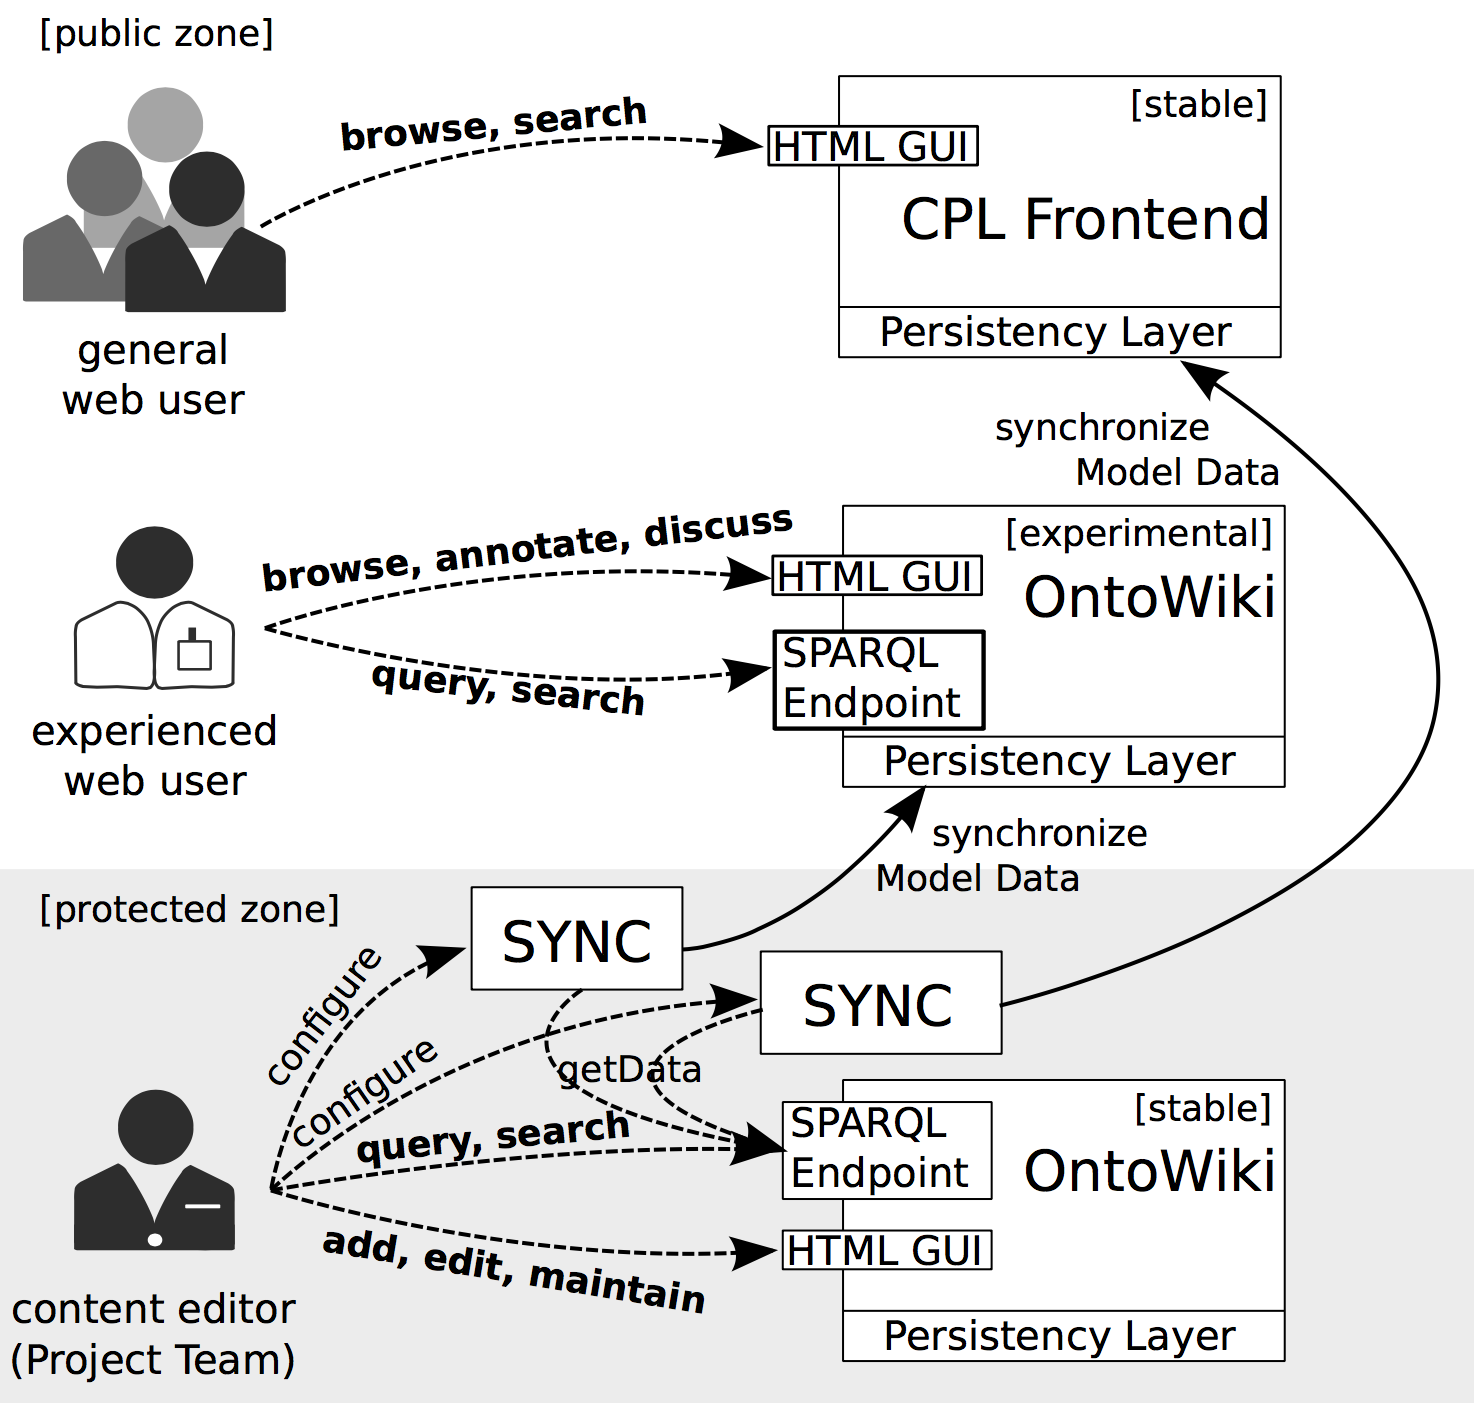
\includegraphics[scale=0.32]{CPL.png}
	\caption{Architecture of Professorenkatalog\cite[p. 6]{dld-paper}}
\end{figure}

}

\frame{

	\frametitle{Simple Docker Demo}
	\framesubtitle{Virtuoso Container}
	
	Virtuoso is a multi model data server including SPARQL RDF based Graph Storage
	\vspace{\baselineskip}
	
	Dockerizing project is hosting an own virtuoso image at:
	
	\begin{center}
		\url{https://registry.hub.docker.com/u/aksw/dld-store-virtuoso7/}
	\end{center}
	
}

\setbeamertemplate{frametitle continuation}{}
\frame[allowframebreaks]{

	\frametitle{Simple Docker Demo}
	\framesubtitle{Run Container}

\begin{center}

	Start and run a docker container through:

	\begin{lstlisting}
	
	docker run -d 
	           --name="virtuoso" 
	           -p <host port>:8890 //SPARQL
	           -p <host port>:1111 //ODBC
                   -e PWDDBA="super secret" 
                   -v <host virtuoso directory>:/var/lib/virtuoso/db
                    aksw/dld-store-virtuoso7

	\end{lstlisting}

\end{center}
}

\setbeamercolor{description item}{fg=blue}
\setbeamercolor{itemize item}{fg=black}

\frame{
	
	\frametitle{Simple Docker Demo}
	\framesubtitle{What is going on?}
	
	\begin{description}
	
	\item[run] Run a command in a new container
	\item[-d] Run container in background and print container ID
	\item[- -name] Assign a name to the container
	\item[-p] Publish a container's port to the host
	\item[-e] Set environment variables into container
	\item[-v] Bind mount a volume
	
	\end{description}
	
	"aksw/dld-store-virtuoso7" is the image name, local or on docker hub

}

\frame{

	\frametitle{Simple Docker Demo}
	\framesubtitle{Setup Virtuoso}

	The virtuoso.ini file is injected into the container through \colorbox{background}{\lstinline{-v}} which mounts the datebase folder from the host system into the container
	\vspace{\baselineskip}
	
	If not specified the container provides a fallback file

}


\frame{

	\frametitle{Simple Docker Demo}
	\framesubtitle{Access Virtuoso Container}

	After \colorbox{background}{\lstinline{docker run}} docker provides an access to the container through the exposed port (\colorbox{background}{\lstinline{-p 8890:8890}}) on localhost
	
	\begin{center}
		\url{http://localhost:8890/sparql}
	\end{center}

}

\frame{

	\begin{figure}
	
	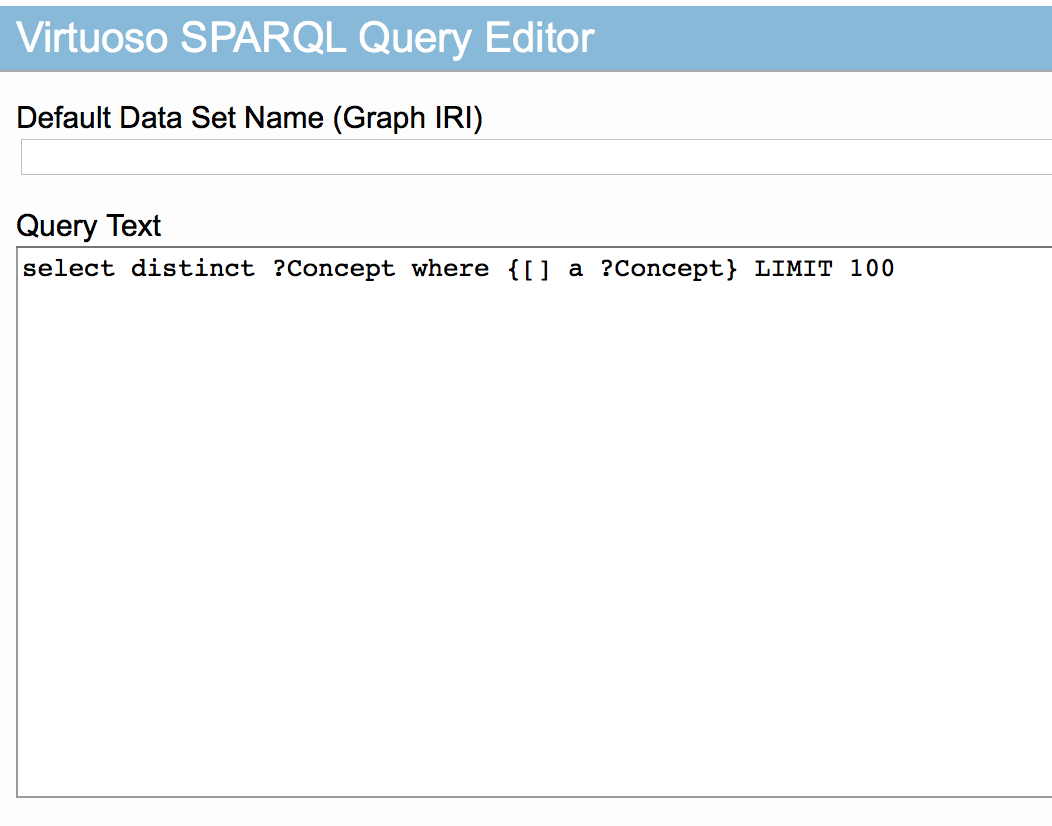
\includegraphics[scale=0.25]{virtuoso-sparql.png}
	\caption{Virtuoso SPARQL Endpoint provided by a docker container}
	
	\end{figure}
}

\frame {
	\frametitle{References}

\begin{thebibliography}{Knowledge Base Shipping to the Linked Open Data Cloud}
	\setbeamertemplate{bibliography item}[text]
      		\bibitem[1]{dld-paper}
        	Knowledge Base Shipping to the Linked Open Data Cloud
 		\newblock {\em Natanael Arndt, Markus Ackermann, Martin Brümmer, Thomas Riechert}
		\newblock{Jul. 2015}
\end{thebibliography}

}

\end{document}
